\subsection{Quality assurance}
To measure the quality of our client and to ensure as few errors as possible, we used the requirements set for the client, along with a test strategy, and the methods described earlier in this chapter.

 The Capability Maturity Model, created by the Software Engineering Institute of Carnegie Mellon University, describes the development process an organization must pass through to be considered mature.
 
 \begin{figure}
 	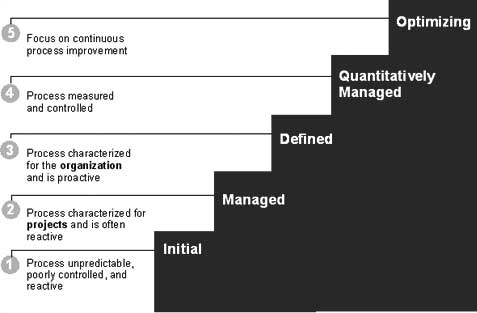
\includegraphics[width=\textwidth]{illustrations/CMM.jpg}
 	\caption{Capability Maturity Model}
 \end{figure}

While doing our project, we moved from the initial level of the Capability Maturity Model (while developing the server) to the managed level (during the development of the client) \cite[p. 242]{PM}. We kept to the initial level during the development of the server, by developing as we went along without using well known development methods or initial design.

The usage of a test strategy, increases the likelihood of finding errors early and correcting them, thereby minimizing the amount of time spend on debugging.
Regarding our project, we decided on a minimal test-strategy. The quality of the program may have suffered from this, but the first part of the project was done without any strategy. The client was better tested than the first part of the project, though we were forced to keep testing at a minimal, due to lack of time.

CISQ, the Consortium for IT Software Quality is comprised by people from different parts of the software industry. It is a neutral forum for customers and suppliers of IT to define, measure and improve IT quality.

If the product fulfills the requirements and pass the tests, its \textbf{reliability} has been proved as well, which is one of CISQ's  major desirable characteristics. The other 4 are; efficiency, security, maintainability and size \cite{CISQ}

\begin{itemize}
	\item Efficiency means that there is minimal to none code duplication, the algorithms are optimized, etc. The code runs as smooth and fast as possible at production.
	\item Security is about how vulnerable the code is to direct attacks. If there are any obvious breaches then they affect this criteria.
	\item Maintainability: How easy is it to understand and edit the product once in production. Documented code and the clear use of known design patterns increases maintainability. 
	\item Size is not a quality indicator per see, but can be used to asses the time needed to complete the product.
\end{itemize}

How our project is measured on these five characteristics:
\begin{itemize}
 	\item The reliability of our server have been a main focus of the group. The server will continue to run after most exceptions, though the server host has been unstable and have had some irregular uptime.
 	\item The efficiency parameter comes partly from our planning and software design and partly from our implementation. We measure this on the algorithms used, are they optimized for performance? Have we planned the development well, by estimated the individual parts well and completing them in a order that minimize development time.
 	\item We have not prioritized security, the server does not encrypt anything. Nor is the connection between the server and client encrypted. We have deliberately chosen this as we found other elements such as streaming, more important. We acknowledge this as unacceptable if it was an actual product.  
 	\item The client is maintainable: We have a well documented and responsibility-driven product, making it easy for others to understand and maintain our code. The server is documented as well, but it is not as transparent as the client.
	\item Size can be used to determine whether we have made it too complicated. If we, from the beginning, had made interfaces for all the modules of our server, we would have seen an overly complex system, but we only discovered this after the server was almost completed. 
\end{itemize}

[ TODO: What are the actual measurable values? And did we meet our goals? ]

During the project's development fase, we had code reviews, first after the server was done. Mainly in order to have everybody understand what the different parts of the server did. In addition it had the effect of illuminating code duplication and poor programming choices.

[ TODO: Update this section when we nearer submission ]